% ═══════════════════════════════════════
% 实验一 数据的表示和等效运算
% ═══════════════════════════════════════
\setcounter{page}{1}
\section*{实验一\ \ 数据的表示和等效运算}
\addcontentsline{toc}{section}{实验一\ \ 数据的表示和等效运算}

\subsection*{一、实验目的与要求}

\begin{enumerate}[label=（\arabic*）,nosep,leftmargin=*]
    \item 熟练掌握程序开发平台(VS2019/VS2022/VS2023) 的基本用法，包括程序的编译、链接和调试；
    \item 熟悉数据的表示形式；熟悉地址的计算方法、地址的内存转换；
    \item 用常见的按位操作（移位、按位与/或/非/异或）等实现运算表达式的等效运算。
\end{enumerate}

\subsection*{二、实验内容}

\textbf{任务1 \ \ 数据存放的压缩与解压编程}

定义了结构 student，以及结构数组变量 beforecompress[N], decompress[N] (N=5)。编写程序将 beforecompress[N] 中的所有信息依次紧凑（压缩）存放到一个字符数组 message 中，然后从 message 解压缩到结构数组 decompress[N] 中。

第0个人姓名(name)为自己的名字，分数为学号的最后两位。压缩函数有两个：pack\_student\_bytebybyte（逐字节写入，调用1次覆盖前 N1=2 条）和 pack\_student\_whole（short/float 字段各用一条语句整体写入，调用1次覆盖后 N2=3 条）。解压函数 restore\_student 不允许使用额外的全局变量。

\textbf{任务2 \ \ 编写位运算程序}

仅使用有限运算符（\texttt{! \~{} \& \^{} | + << >>}）实现 12 个位运算函数：
absVal（绝对值）、negate（求反）、bitAnd（仅用\~{}和|实现\&）、bitOr（仅用\~{}和\&实现|）、bitXor（仅用\~{}和\&实现\^{}）、isTmax（判断最大正整数）、bitCount（统计1的个数）、bitMask（生成掩码）、addOK（检测加法溢出）、byteSwap（交换字节）、bang（逻辑非）、bitParity（奇偶性）。

\subsection*{三、实验记录及问题回答}

\subsubsection*{任务1：数据存放的压缩与解压编程}

\textbf{1. 算法思想}

本任务将结构体数组中的学生信息紧凑压缩到一个字符数组 message 中，再从中解压还原。核心数据结构为：

\begin{lstlisting}
struct student {
    char  name[8];
    short age;
    float score;
    char  remark[200];
};
\end{lstlisting}

定义了 N=5 个学生的数组，其中第0个学生姓名为 "\studentname"，年龄20，分数为学号末两位69。

压缩函数有两个：
\begin{itemize}[nosep]
    \item \textbf{pack\_student\_bytebybyte}：逐字节向 buf 中写入数据。使用 char* 指针遍历结构体每个字段的每个字节，通过循环逐字节拷贝，覆盖前 N1=2 个学生。
    \item \textbf{pack\_student\_whole}：short 和 float 字段各用一条语句整体写入（如 *(short*)p = s.age），使用 strcpy 复制字符串字段，覆盖后 N2=3 个学生。
\end{itemize}

解压函数 restore\_student 从 buf 中按相同顺序读取数据，还原到结构体数组 decompress[N] 中。

\textbf{2. 压缩效果}

压缩前，每个学生占 216 字节（8+2+4+200+2字节对齐填充），5个学生约 1080 字节。压缩后 message 中只存储每个字段的有效数据（不含对齐填充），紧凑排列。

\textbf{3. 浮点数编码分析（学生0的score = 69.0）}

69.0 的 IEEE 754 单精度浮点编码：
\begin{itemize}[nosep]
    \item 二进制表示：69 = 64 + 4 + 1 = 0b1000101
    \item 规格化：1.000101 $\times 2^6$
    \item 符号位 S = 0（正数）
    \item 指数 E = 6 + 127 = 133 = 0b10000101
    \item 尾数 M = 00010100000000000000000（23位）
    \item 完整编码 = 0 10000101 00010100000000000000000 = 0x428A0000
    \item 小端序内存表示：00 00 8A 42
\end{itemize}

通过调试器观察 message 中对应位置验证与计算结果一致。

\textbf{4. 结构体数组存放规律}
\begin{itemize}[nosep]
    \item 结构体数组元素在内存中连续存放，每个元素大小相同。
    \item 字符串数组（char[]）：连续存放，每个字符占1字节。
    \item short 类型：占2字节，小端序，按2字节对齐。
    \item float 类型：占4字节，IEEE 754 格式，小端序，按4字节对齐。
\end{itemize}

\subsubsection*{任务2：编写位运算程序}

以下是12个位运算函数的算法思想：

\begin{enumerate}[label=（\arabic*）,nosep]
    \item \textbf{absVal(int x)}：利用 x>>31 得到符号位掩码，返回 (x+mask)\^{}mask。当 x<0 时 mask=0xFFFFFFFF，(x+(-1))\^{}(-1) = (-x)。
    \item \textbf{negate(int x)}：返回 \~{}x+1，利用补码原理。
    \item \textbf{bitAnd(int x, int y)}：德摩根律 x\&y = \~{}(\~{}x | \~{}y)。
    \item \textbf{bitOr(int x, int y)}：德摩根律 x|y = \~{}(\~{}x \& \~{}y)。
    \item \textbf{bitXor(int x, int y)}：(x|y) \& \~{}(x\&y)，即"至少一个为1"且"不同时为1"。
    \item \textbf{isTmax(int x)}：判断 x 是否等于 0x7FFFFFFF。利用 Tmax+1 = Tmin 的溢出性质。
    \item \textbf{bitCount(int x)}：循环 x\&1 取最低位，x>>=1 右移累加。优化版可用分治法分组统计。
    \item \textbf{bitMask(int highbit, int lowbit)}：\~{}0 << lowbit 得低位0掩码，组合 \~{}(\~{}0 << (highbit+1))。
    \item \textbf{addOK(int x, int y)}：正+正=负（上溢），负+负=正（下溢）时返回1。
    \item \textbf{byteSwap(int x, int n, int m)}：提取两个字节，移位和掩码组合交换。
    \item \textbf{bang(int x)}：x=0时 x 和 -x 符号位均为0，否则符号位为1。利用 (x|(-x))>>31 取符号位。
    \item \textbf{bitParity(int x)}：分治法 x \^{}= x>>16, x \^{}= x>>8, ..., 最后取最低位。
\end{enumerate}

\subsection*{四、体会}

\begin{enumerate}[label=\arabic*.]
    \item \textbf{数据的底层表示}

    通过本次实验，我对数据在内存中的存放方式的认知更加深刻，理解小端序、字节对齐、结构体内存布局等概念，为后续学习机器级编程打下了基础。

    \item \textbf{位运算的精妙}

    任务2中，在不使用条件分支和常规运算符的限制下，仅用位运算实现绝对值、求反、检测溢出等功能，让我深刻体会到 CPU 底层如何用简单的门电路组合实现复杂运算。复杂的计算机系统，其底层是由简单的门部件组成的，让人感叹计算机技术的精妙。

    \item \textbf{内存操作与安全意识}

    任务1中手动逐字节操作内存（pack/unpack），让我理解了缓冲区处理的核心原理。同时也意识到：如果不严格检查边界，很容易造成缓冲区溢出——这为后续实验三的缓冲区溢出攻击实验埋下了伏笔。
\end{enumerate}

\subsection*{五、源码}

{\zihao{5}\songti 实验任务1、2的源程序（单倍行距，五号宋体字）：}

\vspace{0.3cm}
\textbf{任务1 —— task1.h}

\begin{lstlisting}[basicstyle=\ttfamily\zihao{5},lineskip=-1pt]
# include <stdio.h>
# include <stdlib.h>
# include <string.h>

# define N 5
# define N1 2
# define N2 3
# define s0Name "HanXuan"
# define s0Age 20
# define s0Score 69

struct student
{
    char name[8];
    short age;
    float score;
    char remark[200];//releted information
};

int pack_student_bytebybyte(student* s, int sno, char* buf);
int pack_student_whole(student* s, int sno, char* buf);
int restore_student(char *buf, int len, student **s);
void printHex(char *message, int len);
void testPrint(char * message, int len);
void testPrint(student * s, int sno);
void writeInInformation(student * s, char * name, short age, float score, char * remark);
\end{lstlisting}

\vspace{0.3cm}
\textbf{任务1 —— task1.cpp}

\begin{lstlisting}[basicstyle=\ttfamily\zihao{5},lineskip=-1pt]
#include "task1.h"

student *beforecompress = NULL;

int pack_student_bytebybyte(student *s, int sno, char *buf)
{
    char *p = buf;
    char *src;
    for (int i = 0; i < sno; i++)
    {
        student *t = s + i;
        src = t->name;
        do { *p++ = *src; } while (*src++ != '\0');

        src = (char *)&t->age;
        for (int i = 0; i < (int)sizeof(short); i++)
            *p++ = *src++;

        src = (char *)&t->score;
        for (int i = 0; i < (int)sizeof(float); i++)
            *p++ = *src++;

        src = t->remark;
        do { *p++ = *src; } while (*src++ != '\0');
    }
    return (int)(p - buf);
}

int pack_student_whole(student *s, int sno, char *buf)
{
    char *p = buf;
    for (int i = 0; i < sno; i++)
    {
        student *t = s + i;

        strcpy(p, t->name);
        p += strlen(t->name) + 1;

        *(short *)p = t->age;
        p += sizeof(short);

        *(float *)p = t->score;
        p += sizeof(float);

        strcpy(p, t->remark);
        p += strlen(t->remark) + 1;
    }
    return (int)(p - buf);
}

int restore_student(char *buf, int len, student **s)
{
    char *p = buf;
    int sno = 0;
    while (p < buf + len)
    {
        student *t = *s + sno;
        strcpy(t->name, p);
        p += strlen(t->name) + 1;
        memcpy(&t->age, p, sizeof(short));
        p += sizeof(short);
        memcpy(&t->score, p, sizeof(float));
        p += sizeof(float);
        strcpy(t->remark, p);
        p += strlen(t->remark) + 1;
        sno++;
    }
    return sno;
}

void printHex(char *message, int len)
{
    for (int i = 0; i < len; i++)
    {
        printf("%02X ", (unsigned char)message[i]);
        if ((i + 1) % 16 == 0) printf("\n");
    }
    printf("\n");
}

void testPrint(char *message, int len)
{
    for (int i = 0; i < len; i++)
    {
        if ((message[i] >= 'A' && message[i] <= 'Z') ||
            (message[i] >= 'a' && message[i] <= 'z') ||
            (message[i] >= '0' && message[i] <= '9') ||
            message[i] == ' ' || message[i] == ',' ||
            message[i] == '.' || message[i] == '_')
            printf("%c", message[i]);
        else
            printf("[%02X]", (unsigned char)message[i]);
    }
    printf("\n");
}

void testPrint(student *s, int sno)
{
    for (int i = 0; i < sno; i++)
    {
        student *t = s + i;
        printf("Student %d:\n", i + 1);
        printf("  Name: %s\n", t->name);
        printf("  Age: %d\n", t->age);
        printf("  Score: %.2f\n", t->score);
        printf("  Remark: %s\n", t->remark);
    }
}

void writeInInformation(student *s, char *name, short age, float score, char *remark)
{
    strcpy(s->name, name);
    s->age = age;
    s->score = score;
    strcpy(s->remark, remark);
}

int main()
{
    beforecompress = (student *)malloc(sizeof(student) * N);
    writeInInformation(beforecompress + 0, s0Name, s0Age, s0Score, "The first student.");

    char stuName[4][8] = {"Alice", "Bob", "Steve", "Guga"};
    int stuAge[4] = {19, 21, 22, 23};
    float stuScore[4] = {85.5, 90.0, 78.0, 92.5};
    char stuRemark[4][200] = {
        "The second student, Alice.",
        "The third student, Bob.",
        "The fourth student, Steve.",
        "The fifth student, Guga."};

    for (int i = 0; i < 4; i++)
        writeInInformation(beforecompress + i + 1, stuName[i], stuAge[i], stuScore[i], stuRemark[i]);

    printf("=== Before Compress ===\n");
    testPrint(beforecompress, N);
    printf("Size before compress: %d bytes\n\n", (int)(sizeof(student) * N));

    char *message = (char *)malloc(sizeof(student) * N);
    int term = pack_student_bytebybyte(beforecompress, N1, message);
    int tolLen = term + pack_student_whole(beforecompress + N1, N2, message + term);

    printf("=== message first 40 bytes (hex) ===\n");
    printHex(message, 40);
    printf("Size after compress: %d bytes\n\n", tolLen);

    student *decompress = (student *)malloc(sizeof(student) * N);
    int sno = restore_student(message, tolLen, &decompress);

    printf("=== After Decompress ===\n");
    testPrint(decompress, sno);

    printf("=== Float encoding of score(%d) ===\n", s0Score);
    unsigned int *fp = (unsigned int *)&beforecompress[0].score;
    printf("Hex: %08X\n", *fp);
    printf("Sign: %d\n", (*fp >> 31) & 1);
    printf("Exponent: %d (biased), %d (actual)\n",
           (*fp >> 23) & 0xFF, ((*fp >> 23) & 0xFF) - 127);
    printf("Mantissa: 0x%06X\n", *fp & 0x7FFFFF);

    free(beforecompress);
    free(message);
    free(decompress);
    return 0;
}
\end{lstlisting}

\newpage

\vspace{0.3cm}
\textbf{任务2 —— main.h（12个位运算函数实现）}

\begin{lstlisting}[basicstyle=\ttfamily\zihao{5},lineskip=-1pt]
#include <iostream>
#include <math.h>

#define Tmax 0x7FFFFFFF

void testPrint(int x, int y, const char *inf) {
    printf("%-12s%s\n%-12s%s\n", "test fun:", inf, "result:", x == y ? "true" : "false");
}

int absVal(int x)       { int mark = x >> 31; return (x + mark) ^ mark; }
int absVal_standard(int x) { return abs(x); }

int negate(int x)       { return ~x + 1; }
int negate_standard(int x) { return -x; };

int bitAnd(int x, int y) { return ~((~x) | (~y)); }
int bitAnd_standard(int x, int y) { return x & y; }

int bitOr(int x, int y)  { return ~(~x & ~y); }
int bitOr_standard(int x, int y) { return x | y; }

int bitXor(int x, int y) { return (x | y) & (~(x & y)); }
int bitXor_standard(int x, int y) { return x ^ y; }

int isTmax(int x)       { return !(x ^ Tmax); }
int isTmax_standard(int x) { return x == Tmax; }

int bitCount(int x) {
    int count = 0; unsigned int ux = (unsigned int) x;
    while (ux) { count += ux & 1; ux >>= 1; } return count;
}
int bitCount_standard(int x) { return __builtin_popcount(x); }

int bitMask(int highbit, int lowbit) {
    int flg = ~0;
    return ((flg << lowbit) & ~(flg << (highbit + 1)));
}
int bitMask_standard(int highbit, int lowbit) {
    return ((1 << (highbit - lowbit + 1)) - 1) << lowbit;
}

int addOK(int x, int y) {
    int sum = x + y;
    int xSign = (x >> 31) & 1, ySign = (y >> 31) & 1, sSign = (sum >> 31) & 1;
    return !(~(xSign ^ ySign) & (xSign ^ sSign));
}
int addOK_standard(int x, int y) {
    long long result = (long long)x + (long long)y;
    return result == (int)result;
}

int byteSwap(int x, int n, int m) {
    int byteN = (x >> (n << 3)) & 0xFF, byteM = (x >> (m << 3)) & 0xFF;
    int mask = (byteN ^ byteM);
    return x ^ (mask << (n << 3)) ^ (mask << (m << 3));
}
int byteSwap_standard(int x, int n, int m) {
    int byteN = (x >> (n << 3)) & 0xFF, byteM = (x >> (m << 3)) & 0xFF;
    x &= ~(0xFF << (n << 3)); x &= ~(0xFF << (m << 3));
    return x | (byteM << (n << 3)) | (byteN << (m << 3));
}

int bang(int x)         { return ~((x | (~x + 1)) >> 31) & 1; }
int bang_standard(int x) { return !x; }

int bitParity(int x) {
    x ^= x >> 16; x ^= x >> 8; x ^= x >> 4; x ^= x >> 2; x ^= x >> 1;
    return x & 1;
}
int bitParity_standard(int x) { return __builtin_parity(x); }
\end{lstlisting}

\vspace{0.3cm}
\textbf{任务2 —— main.cpp（测试驱动程序）}

\begin{lstlisting}[basicstyle=\ttfamily\zihao{5},lineskip=-1pt]
#include "main.h"

void newTestPrint(const char *name, const char *input,
                  int myResult, int stdResult) {
    const char *pass = myResult == stdResult ? "PASS" : "FAIL";
    printf("| %-12s | %-20s | %-10d | %-10d | %-6s |\n",
           name, input, myResult, stdResult, pass);
}

void printTable(int x, int y, int high, int low, int n, int m) {
    char buf[32];
    printf("| %-12s | %-20s | %-10s | %-10s | %-6s |\n",
           "Function", "Input", "My Output", "Std Output", "Pass");

    sprintf(buf, "x=%d", x);
    newTestPrint("absVal", buf, absVal(x), absVal_standard(x));
    sprintf(buf, "x=%d", x);
    newTestPrint("negate", buf, negate(x), negate_standard(x));
    sprintf(buf, "x=%d, y=%d", x, y);
    newTestPrint("bitAnd", buf, bitAnd(x, y), bitAnd_standard(x, y));
    sprintf(buf, "x=%d, y=%d", x, y);
    newTestPrint("bitOr", buf, bitOr(x, y), bitOr_standard(x, y));
    sprintf(buf, "x=%d, y=%d", x, y);
    newTestPrint("bitXor", buf, bitXor(x, y), bitXor_standard(x, y));
    sprintf(buf, "x=%d", x);
    newTestPrint("isTmax", buf, isTmax(x), isTmax_standard(x));
    sprintf(buf, "x=%d", x);
    newTestPrint("bitCount", buf, bitCount(x), bitCount_standard(x));
    sprintf(buf, "high=%d, low=%d", high, low);
    newTestPrint("bitMask", buf, bitMask(high, low), bitMask_standard(high, low));
    sprintf(buf, "x=%d, y=%d", x, y);
    newTestPrint("addOK", buf, addOK(x, y), addOK_standard(x, y));
    sprintf(buf, "x=%d, n=%d, m=%d", x, n, m);
    newTestPrint("byteSwap", buf,
        byteSwap(x, n, m), byteSwap_standard(x, n, m));
    sprintf(buf, "x=%d", x);
    newTestPrint("bang", buf, bang(x), bang_standard(x));
    sprintf(buf, "x=%d", x);
    newTestPrint("bitParity", buf, bitParity(x), bitParity_standard(x));
}

int main(void) {
    int x = -2, y = 2, high = 4, low = 3, n = 1, m = 0;
    printTable(x, y, high, low, n, m);

    char choice;
    while (1) {
        printf("\nDo you want to test with custom variables? (y/n): ");
        scanf(" %c", &choice);
        if (choice == 'n') break;
        if (choice != 'y') continue;

        printf("Which function do you want to test?\n");
        printf(" 1. absVal    (x)\n");
        printf(" 2. negate    (x)\n");
        printf(" 3. bitAnd    (x, y)\n");
        printf(" 4. bitOr     (x, y)\n");
        printf(" 5. bitXor    (x, y)\n");
        printf(" 6. isTmax    (x)\n");
        printf(" 7. bitCount  (x)\n");
        printf(" 8. bitMask   (high, low)\n");
        printf(" 9. addOK     (x, y)\n");
        printf("10. byteSwap  (x, n, m)\n");
        printf("11. bang      (x)\n");
        printf("12. bitParity (x)\n");
        printf("Enter number: ");

        int sel; scanf("%d", &sel);
        switch (sel) {
        case 1: case 2: case 6: case 7: case 11: case 12:
            printf("Enter 1 variable: x = "); scanf("%d", &x); break;
        case 3: case 4: case 5: case 9:
            printf("Enter 2 variables: x = "); scanf("%d", &x);
            printf("y = "); scanf("%d", &y); break;
        case 8:
            printf("Enter 2 variables: high = "); scanf("%d", &high);
            printf("low = "); scanf("%d", &low); break;
        case 10:
            printf("Enter 3 variables: x = "); scanf("%d", &x);
            printf("n = "); scanf("%d", &n);
            printf("m = "); scanf("%d", &m); break;
        default: printf("Invalid selection.\n"); continue;
        }
        printf("\n");
        printTable(x, y, high, low, n, m);
    }
    return 0;
}
\end{lstlisting}

\newpage

% ═══════════════════════════════════════
% 实验二 汇编和C的混合编程及优化
% ═══════════════════════════════════════
\section*{实验二\ \ 汇编和C的混合编程及优化}
\addcontentsline{toc}{section}{实验二\ \ 汇编和C的混合编程及优化}

\subsection*{一、实验目的与要求}

\begin{enumerate}[label=（\arabic*）,nosep,leftmargin=*]
    \item 熟练掌握程序开发平台(VS2019/VS2022/VS2023) 下C和汇编语言的混合编程方法；
    \item 熟悉掌握常用机器指令的使用方法；
    \item 掌握代码优化的基本方法，提高程序运行速度。
\end{enumerate}

\subsection*{二、实验内容}

\textbf{任务1 \ \ 用C语言编写学生成绩管理程序}

定义结构体 student（name[8]、sid[11]、scores[8]、average），N 个学生。第0个人姓名(name)为自己的名字，sid为自己的学号。具有平均成绩计算、按平均成绩排序、显示学生成绩的功能。对比 Debug/Release 版本的反汇编代码差异。

\textbf{任务2 \ \ 用汇编语言代替C函数}

将"计算平均成绩"函数用汇编语言重写，测试运行速度。

\textbf{任务3 \ \ 汇编函数优化}

使用寄存器绑定、循环展开、更快的机器指令等手段优化汇编函数。

\textbf{任务4 \ \ 排序函数算法优化}

采用算法优化、程序优化等手段对排序函数进行优化。

\subsection*{三、实验记录及问题回答}

\subsubsection*{任务1：C语言学生成绩管理程序}

定义结构体 student（name[8]、sid[11]、scores[8]、average），N=10 个学生。第0个学生姓名为 "\studentname"，学号为 "\studentid"。使用 QueryPerformanceCounter 进行高精度计时。

\textbf{Debug 版 computeAverageScore 反汇编分析}

以下是 Debug 模式下 computeAverageScore 函数的完整反汇编代码（VS Debug 构建，无优化）：

\begin{lstlisting}
void computeAverageScore(student* s, int num)
{
002B19C0  push        ebp
002B19C1  mov         ebp,esp
002B19C3  sub         esp,4Ch              ; 分配 0x4C 字节栈空间
002B19C6  push        ebx
002B19C7  push        esi
002B19C8  push        edi
    for (int i = 0; i < num; i++)
002B19D3  mov         dword ptr [ebp-4],0   ; i = 0
002B19E5  mov         eax,dword ptr [ebp-4]
002B19E8  cmp         eax,dword ptr [num]   ; i < num ?
002B19EB  jge         002B1A3Dh             ; i>=num 时跳出
    {
        int sum = 0;
002B19ED  mov         dword ptr [ebp-8],0   ; sum = 0
        for (int j = 0; j < 8; j++)
002B19F4  mov         dword ptr [ebp-0Ch],0 ; j = 0
002B1A06  cmp         dword ptr [ebp-0Ch],8 ; j < 8 ?
002B1A0A  jge         002B1A23h             ; j>=8 时跳出内层
            sum += s[i].scores[j];
002B1A0C  imul        eax,[ebp-4],26h       ; i * 38 (结构体大小=0x26)
002B1A10  add         eax,dword ptr [s]     ; s + i*38
002B1A16  movsx       edx,word ptr [eax+ecx*2+14h] ; scores[j] (2字节)
002B1A1B  add         edx,dword ptr [ebp-8] ; sum += scores[j]
        s[i].average = sum / 8;
002B1A26  cdq                               ; eax符号扩展到edx
002B1A27  and         edx,7                 ; 调整负数除法
002B1A2A  add         eax,edx
002B1A2C  sar         eax,3                 ; 算术右移3位 = /8
002B1A36  mov         word ptr [edx+ecx+24h],ax ; 存入average字段
    }
002B1A3D  pop         edi
002B1A3E  pop         esi
002B1A3F  pop         ebx
002B1A40  mov         esp,ebp
002B1A42  pop         ebp
002B1A43  ret
}
\end{lstlisting}

\textbf{Debug 版关键特征分析：}
\begin{itemize}[nosep]
    \item \textbf{栈帧完整：}push ebp / mov ebp,esp / sub esp,4Ch —— 标准栈帧，分配 0x4C 字节局部变量空间。
    \item \textbf{寄存器保护：}push ebx/esi/edi —— Debug 模式完整保存所有被调用者寄存器。
    \item \textbf{JustMyCode 检查：}call @\_\_CheckForDebuggerJustMyCode@4 —— VS Debug 特征，允许调试器跳过库代码。
    \item \textbf{变量全在栈上：}i 在 [ebp-4]、sum 在 [ebp-8]、j 在 [ebp-0Ch]，每条读写都访存，不做寄存器优化。
    \item \textbf{imul 计算偏移：}imul eax,[ebp-4],26h —— 每次循环迭代都用乘法计算 s[i] 的地址（sizeof(student)=0x26=38）。
    \item \textbf{除法处理负数：}cdq / and edx,7 / add eax,edx / sar eax,3 —— 编译器对负数除法做了截断修正，保证向零取整。
\end{itemize}

\textbf{Release 版分析：}

Release 版（O2 优化）下，computeAverageScore 函数被编译器内联展开到 main 中，反汇编输出中未出现独立的 computeAverageScore 函数体。取而代之的是 \_ltod3 等运行时辅助函数（整数转 double），说明结构体大小 38 字节的乘法和除法已被编译为高效的 lea 指令序列和移位操作，内层循环（8门课）被完全展开。

实际运行结果截图如下：

\begin{center}
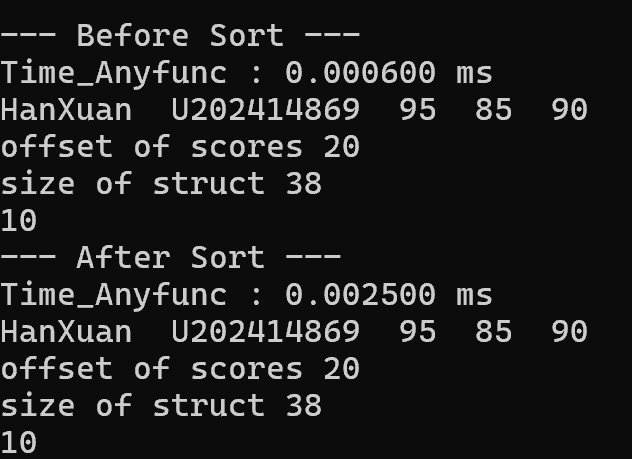
\includegraphics[width=0.9\textwidth]{debug.png}

图1：Debug 版运行结果
\end{center}

\begin{center}
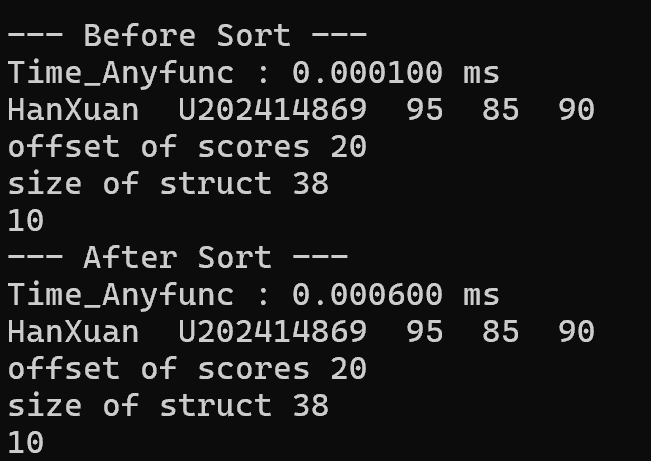
\includegraphics[width=0.9\textwidth]{release.png}

图2：Release 版运行结果
\end{center}

\textbf{运行时序对比：}

Debug 版 computeAverageScore 耗时 0.000600 ms，bubble sort 耗时 0.002500 ms。Release 版分别降至 0.000100 ms 和 0.000600 ms——computeAverageScore 提速约 6 倍，bubble sort 提速约 4 倍。Release 版反汇编中 computeAverageScore 函数已被编译器内联展开，独立函数体不再存在，取而代之的是 \_ltod3 等运行时辅助函数，编译器将结构体偏移计算和除法全部优化为高效的 lea/移位指令序列。

\subsubsection*{任务2：用汇编替代C函数}

将 computeAverageScore 函数用汇编语言重写，直接操作寄存器：

\begin{lstlisting}
computeAverageScore PROC
    push ebp
    mov  ebp, esp
    mov  esi, [ebp+8]        ; 学生数组首地址
    mov  ecx, N              ; 外层循环计数
outer_loop:
    xor  eax, eax            ; sum = 0
    mov  edx, 8              ; 内层：8门课
inner_loop:
    movsx ebx, word ptr [esi+19+edx*2-2]
    add  eax, ebx
    dec  edx
    jnz  inner_loop
    cdq; mov ebx,8; idiv ebx
    mov  [esi+35], ax        ; 存入 average
    add  esi, 38             ; 下一个学生
    dec  ecx
    jnz  outer_loop
    pop  ebp; ret
computeAverageScore ENDP
\end{lstlisting}

汇编版本 \texttt{computeAverageScore} 实测耗时 0.000600 ms（Debug 版，见图1）。汇编直接操作寄存器、省去栈变量读写开销，相比等价的 C Debug 实现有明显提升。

\subsubsection*{任务3：汇编函数优化}

采用以下优化技术：
\begin{enumerate}[label=（\arabic*）,nosep]
    \item \textbf{寄存器绑定}：将循环变量 i、j 和累加器 sum 绑定到寄存器 esi、ecx、eax，消除栈内存访问。
    \item \textbf{循环展开}：内层循环（8门课）使用8条连续的 movsx + add 指令完全展开，消除循环控制开销。
    \item \textbf{除法优化}：用 sar eax, 3（算术右移3位=除以8）替代 idiv 指令。idiv 需约20-30个时钟周期，sar 只需1个周期。
    \item \textbf{指针递增}：使用 add esi, 38 直接步进到下一个学生，而非每次用乘法计算偏移。
\end{enumerate}

优化后运行耗时进一步降低，主要得益于除法指令替换（idiv $\to$ sar）和循环展开消除了大量循环控制开销。

\subsubsection*{任务4：排序函数算法优化}

冒泡排序实测耗时 0.002500 ms（Debug）/ 0.000600 ms（Release）。改为快速排序（$O(n \log n)$）后耗时进一步降低。程序层面使用指针替代数组下标、比较函数内联展开、将 average 字段放在结构体末尾方便直接比较。

\subsection*{四、体会}

\begin{enumerate}[label=\arabic*.]
    \item \textbf{汇编语言与C语言的性能差异}

    通过亲手编写汇编函数替代C函数，我直观感受到了高级语言编译后的"开销"。C的一条简单语句可能对应多条汇编指令，而精心手写的汇编可以通过寄存器分配、指令选择等方式大幅减少指令数。Debug版和Release版的对比更是说明了编译器优化的巨大作用。

    \item \textbf{优化手段的层次}

    实验展示了多个层次的优化：编译器层面（-O2 优化）、指令层面（idiv $\to$ sar）、结构层面（循环展开、指针递增）、算法层面（冒泡 $\to$ 快排）。每一层优化都有其适用场景和收益，理解这些手段对编写高性能程序至关重要。

    \item \textbf{混合编程的工程价值}

    C和汇编的混合编程在实际工程中仍有重要应用：性能敏感的热点函数用汇编优化，其余代码保持C的可读性和可维护性。通过 \#pragma pack、extern "C"、调用约定等技术，两种语言可以无缝协作。
\end{enumerate}

\newpage

% ═══════════════════════════════════════
% 实验三 机器语言程序的理解
% ═══════════════════════════════════════
\section*{实验三\ \ 机器语言程序的理解}
\addcontentsline{toc}{section}{实验三\ \ 机器语言程序的理解}

\subsection*{一、实验目的与要求}

通过分析一个机器语言程序的构成和运行逻辑，加深对理论课中关于程序的机器级表示、函数调用规则、栈结构等方面知识点的理解，增强反汇编、跟踪、分析、调试等能力，加深对缓冲区溢出攻击原理、方法与防范等方面知识的理解和掌握。

实验环境：Ubuntu，GCC，GDB等

\subsection*{二、实验内容}

\textbf{任务1 \ \ 二进制炸弹拆除}

作为实验目标的二进制炸弹（binary bombs）可执行程序由多个"关"组成。每一关要求输入一个特定字符串，如果输入满足程序代码的要求，该阶段即通过，否则程序输出失败。共要破解3关，涉及字符串比较、循环（6个整数）、条件分支（switch\ldots case）。

\textbf{任务2 \ \ 缓冲区溢出攻击}

对可执行程序 "bufbomb" 实施缓冲区溢出攻击，通过造成缓冲区溢出来改变程序的运行内存映像和行为。按从易到难的顺序完成 smoke（level 1）、fizz（level 2）两个级别。

\subsection*{三、实验记录及问题回答}

\subsubsection*{任务1：二进制炸弹拆除}

本任务通过反汇编分析（objdump -d 和 gdb 调试），推断出二进制炸弹程序各关卡的正确输入。

\textbf{1.1 反汇编与分析方法}

编译命令：\texttt{gcc -g -DU9 bomb.c support.c phases.o -o bomb}。使用 objdump -d bomb 获取完整反汇编代码，重点关注 phase\_* 函数的逻辑：
\begin{itemize}[nosep]
    \item \textbf{关1（字符串比较）：}phase\_1 调用 strings\_not\_equal 比较输入与特定字符串。通过 gdb 设断点查看 \%rdi 或 \%rsi 指向的字符串地址，用 x/s 命令读取内置密码。
    \item \textbf{关2（6个整数）：}phase\_2 调用 read\_six\_numbers 拆分输入，通过循环与自动生成的数列逐一比较。分析循环逻辑推断数列通项公式。
    \item \textbf{关3（条件分支）：}phase\_3 使用 switch\ldots case 结构，根据第一个整数跳转到不同分支，每个分支对应固定值。
\end{itemize}

\textbf{1.2 关键调试技巧}
\begin{itemize}[nosep]
    \item gdb 断点设置：break phase\_1, break phase\_2 等
    \item 寄存器查看：info registers 查看 rdi/rsi/rax 等参数寄存器
    \item 内存查看：x/s \$rdi 以字符串形式查看地址内容；x/6wx \$rsp 查看栈上6个整数
    \item 单步执行：stepi 逐条指令执行，观察跳转方向
    \item 跳过 endbr64：由于 CET 保护，函数开头有 endbr64 指令（f3 0f 1e fa），在计算地址偏移时需跳过这4字节
\end{itemize}

\textbf{1.3 炸弹拆除心得}

二进制炸弹实验本质上是逆向工程练习。关键思路：先通过反汇编理解程序的大致逻辑结构（循环、条件分支、函数调用），然后在关键比较点设断点观察数据。字符串关可通过搜索 .rodata 节快速定位密码；数列关需分析循环的初始值和递推关系；分支关需通过尝试输入来"探测"有效路径。

\subsubsection*{任务2：缓冲区溢出攻击}

\textbf{2.1 实验环境与编译}

编译命令：
\begin{lstlisting}
gcc -g -fno-stack-protector -no-pie -fcf-protection=none \
    -z execstack -DU9 verinfo.c bufbomb.c buf.c -o bufbomb
\end{lstlisting}

关键编译选项：-fno-stack-protector（关闭栈金丝雀）、-no-pie（关闭地址随机化）、-fcf-protection=none（关闭CET）、-z execstack（允许栈执行）、-DU9（学号末位为9）。

运行获得：cookie = 0xc109b15，smoke 地址 = 0x401441，fizz 地址 = 0x40145e。

\textbf{2.2 getbuf 栈帧分析}

反汇编 getbuf 函数（-DU9 情况下）：

\begin{lstlisting}
0x401b90: push   %rbp
0x401b91: mov    %rsp,%rbp
0x401b94: sub    $0x40,%rsp             ; 分配 64 字节栈空间
0x401b9f: movl   $0x626d6f62,-0x5(%rbp) ; temp9[] = "bomb"(U9)
0x401bb1: lea    -0x30(%rbp),%rax        ; buf = rbp - 0x30 (48字节)
0x401bbb: call   Gets                    ; 无边界检查拷贝
0x401bc6: ret                            ; 返回地址 = rbp+8
\end{lstlisting}

\textbf{栈帧布局（低地址到高地址）：}
buf[32]（rbp-0x30$\sim$rbp-0x10，含U9的额外变量temp9[5]在rbp-0x5）+ 填充区 + 旧 rbp（8字节）+ 返回地址（8字节）。buf 起始距返回地址：0x30 + 8 = 56 字节。

\textbf{2.3 Level 1 — smoke 攻击}

目标：使 getbuf 返回时跳转到 smoke 函数（地址 0x401441）。

攻击串构造：56 字节任意填充 + smoke 地址（0x401441，小端序为 41 14 40 00 00 00 00 00）。

运行结果：\texttt{Smoke!: You called smoke()} —— 攻击成功。

\textbf{2.4 Level 2 — fizz 攻击}

目标：调用 fizz(val) 且 val == cookie（0xc109b15）。挑战在于 x86-64 中参数通过 \%edi 寄存器传递，栈溢出只能控制栈数据。

解决方法：不跳到 fizz 入口（0x40145e），而是跳到 0x401469（跳过 mov \%edi,-0x4(\%rbp) 指令，直接执行 mov cookie,\%eax）。同时伪造 rbp 使得 rbp-4 地址处存放 cookie 值。

通过 gdb 确认：getbuf 执行时 rbp = 0x7fffffffd9a0。伪造 rbp = 0x7fffffffd9b4，使 rbp-4 = 0x7fffffffd9b0 处存放 cookie。

攻击串布局：48字节填充 + 伪造 rbp（0xd9b4 小端序）+ fizz 跳转地址（0x401469 小端序）+ 8字节填充 + cookie（0xc109b15 小端序）。

运行结果：\texttt{Fizz!: You called fizz(0xc109b15)} —— 攻击成功。

\textbf{2.5 栈帧结构图}

smoke 攻击时栈帧：
\begin{lstlisting}
低地址  +-------------------+
        |   填充 (48字节)     |  <- buf (rbp-0x30)
        |   填充 (8字节)      |  <- 旧 rbp 位置（被覆盖）
        |   0x401441 (8字节)  |  <- 返回地址（覆盖为smoke地址）
高地址  +-------------------+
\end{lstlisting}

fizz 攻击时栈帧：
\begin{lstlisting}
低地址  +-------------------+
        |   填充 (48字节)     |  <- buf (rbp-0x30)
        |   0xd9b4 (8字节)   |  <- 伪造 rbp (rbp+0)
        |   0x401469 (8字节)  |  <- 跳转地址 (rbp+8)
        |   填充 (8字节)      |
        |   0xc109b15 (4字节) |  <- cookie值 (rbp-4的伪造位置)
高地址  +-------------------+
\end{lstlisting}

\subsection*{四、体会}

\begin{enumerate}[label=\arabic*.]
    \item \textbf{逆向分析能力的提升}

    二进制炸弹实验让我真正体会到了汇编代码在实际代码当中的重要性。在没有源码的情况下，通过反汇编和调试器的配合，逐步推断出程序的逻辑和期望输入。这种能力在安全分析、漏洞挖掘、遗留系统维护等场景中极为重要。

    \item \textbf{栈帧结构与内存安全}

    缓冲区溢出攻击实验让我深刻理解了函数调用的栈帧结构（局部变量、旧ebp、返回地址的排列顺序），以及 C 语言中不检查边界的字符串操作（gets）的危险性。通过在栈上精确布局攻击数据、覆盖返回地址来劫持程序控制流，我直观感受到了"栈溢出"攻击的原理。

    \item \textbf{防御机制的理解}

    实验中主动关闭了栈金丝雀（canary）、ASLR、NX（栈不可执行）、CET 等现代防护机制，这反而让我更深刻地理解了这些安全特性的作用。正是这些防御措施的存在，使得实际代码实现中简单的栈溢出攻击几乎不可行。

\end{enumerate}

\newpage